\documentclass[ngerman,landscape,twocolumn]{adtexsheet}

 %for pseudocode
 %http://tug.ctan.org/macros/latex/contrib/algorithm2e/doc/algorithm2e.pdf
\usepackage[ruled,noend,noline,nofillcomment,linesnumbered,]{algorithm2e}
\DontPrintSemicolon
\SetKwFor{For}{for }{}{}
\SetKwFor{While}{while }{}{}
\SetKwIF{If}{ElseIf}{Else}{if}{}{else if}{else}{}
\SetKw{Return}{return}
\newcommand{\To}{\KwTo}
\newcommand{\swap}{\leftrightarrow}
\newcommand*{\CommentInLine}{\tcc*[f]}
\newcommand{\todo}{\colorbox{red}{\textbf{Muss noch was gemacht werden}}}
\usepackage{mathtools}
\DeclarePairedDelimiter\ceil{\lceil}{\rceil}
\DeclarePairedDelimiter\floor{\lfloor}{\rfloor}
\DeclarePairedDelimiter\abs{|}{|}

\exnumber{5}
%Teilnehmer
%<Name> & <Gruppennummer> & <Kreuz Aufgabe 1> & <Kreuz Aufgabe 2> & <Kreuz Aufgabe 3> & <Kreuz Aufgabe 4>
\participantOne{Theodor Bajusz&5&x&x&x&x&x}
\participantTwo{Valerij Dobler&13&x&x&x&x&x}
\participantThree{Matz Radloff&6&x&x&x&x&x}
\participantFour{Robin Wannags&5&x&x&x&x&x}

% sheet specific notions and notation,
%drawing automatons
\usepackage{tikz}
\usetikzlibrary{shapes}
\usepackage{listings}
\usepackage{stmaryrd}

\begin{document}

\begin{question}
    Gegeben ist eine Hashtabelle $T$ der Länge $m = 11$ mit Hashfunktion $h(k;i) = (k + i^2)\,mod\,m$. Tragen Sie die Schlüssel $56, 46, 31, 45,42, 65, 29, 44, 23$ in der angegebenen Reihenfolge in die Hashtabelle ein. Verwalten Sie Kollisionen:
    \begin{enumerate}
        \item durch Verkettung (i = 0), (2 Punkte)
        \item durch offene Adressierung. (2 Punkte)
        
        \begin{table}[]
            \centering
            \newcommand{\sep}{\rightarrow}
            \subfloat[\centering durch Verkettung]
            {{
            \begin{tabular}{c|l}
                Index & Verkettete Liste \\\hline 
                 $0$ & $\fbox{44}$\\
                 $1$ & $\fbox{23} \sep \fbox{45} \sep \fbox{56}$\\
                 $2$ & $\fbox{46}$\\
                 $3$ & \\
                 $4$ & \\
                 $5$ & \\
                 $6$ & \\
                 $7$ & $\fbox{29}$\\
                 $8$ & \\
                 $9$ & $\fbox{42} \sep \fbox{31}$\\
                 $10$& $\fbox{65}$\\
            \end{tabular}
            }}%
            \qquad
            \subfloat[\centering offene Adressierung]{{
            \begin{tabular}{c|l}
                Index & Elemente \\\hline 
                 $0$ & $\fbox{65}$\\
                 $1$ & $\fbox{56}$\\
                 $2$ & $\fbox{46}$\\
                 $3$ & \\
                 $4$ & $\fbox{44}$\\
                 $5$ & $\fbox{45}$\\
                 $6$ & $\fbox{23}$\\
                 $7$ & $\fbox{29}$\\
                 $8$ & \\
                 $9$ & $\fbox{31}$\\
                 $10$& $\fbox{42}$\\
            \end{tabular}
            }}%
        \end{table}
    \end{enumerate}
\end{question}

\begin{question}
    \begin{enumerate}
        \item Nehmen Sie an, die Suche nach einem Schlüssel $k$ in einem binären Suchbaum endet in einem Blatt. Dann gibt es drei Mengen: $A$, die Schlüssel links des Suchpfads; $B$, die Schlüssel auf dem Suchpfad; sowie $C$, die Schlüssel rechts des Suchpfads. Beweisen oder widerlegen Sie die folgende Behauptung: Für beliebige drei Schlüssel $a \in A, b \in B$ und $c \in C$ gilt $a \leq b \leq c$. (2 Punkte)
        
        \emph{Behauptung:} Seien $B$ und $C$ wie oben definiert, dann gilt $$\forall b \in B \forall c \in C: b \leq c$$
        \begin{proof} Sei der Suchbaum wie folgt
        \begin{center}
            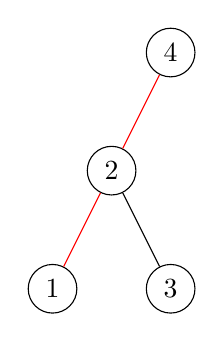
\begin{tikzpicture}[every node/.style={circle,draw=black}]
            \node{4}[draw=red]
                child { node{2}
                    child { node{1} }
                    child[black] { node{3} }
                }
                child[missing] {}
            ;
            \end{tikzpicture}
        \end{center}
        und $1$ der gesuchte Wert. Dann sehen die Mengen so aus: 
\[
A=\emptyset, \quad B=\{4,2,1\}, \quad C=\{3\}
\]
        Hierbei ist $4 \in B \land 3 \in C$ aber $4 > 3$ ist, was einen Widerspruch zur Behauptung liefert.
        \end{proof}
        
        \newpage
        \item Aus der Vorlesung ist Ihnen bekannt, dass zum Suchen in einem vollständigen Binärbaum $O(log_2\,n)$ Zeit benötigt wird. Wie ist die asymptotische Laufzeit, wenn stattdessen jeder innere Knoten bis zu $3$ Kinder haben darf? Wie, bei bis zu $log_2\,n$ Kindern? (2 Punkte)
        
        \begin{behauptung}
        Ein ternärer Suchbaum ist ein Suchbaum bei dem jeder innere Knoten bis zu $3$ Kindern haben kann. Die Suche in so einem vollständigen Baum benötigt $O(log_2\, n)$ Zeit.
        \end{behauptung}
        \begin{proof}
        In einem ternären Baum muss man pro Knoten bis zu $2$ Vergleiche machen um entscheiden zu können, in welchem Kind man weiter suchen muss. Ideal balanciert, würde dessen Höhe $\ceil*{log_3\,n}$ betragen. In einem vollständigen ternären Suchbaum würde die Suche folglich
\[
O(2 \cdot log_3\,n) = O\left(2 \cdot \frac{log_2\, n}{log_2\, 3}\right) = O(log_2\, n)
\]
        Zeit benötigen.
        \end{proof}
        
        Teil zwei. Die Höhe eines solchen Suchbaumes wächst in $O(log_2(n))$ und die Anzahl der nötigen Vergleiche pro Knoten wächst auch in Abhängigkeit von $O(log_2(n))$. Für die Laufzeit der Suche ergibt sich dann:
\[
O\left(log_{log_2(n)}(n) \cdot log_2(n)\right)
.\]
    \end{enumerate}
\end{question}


\begin{question}
    Sei n die Anzahl der Knoten im Baum, und h die Höhe des Baumes.
    \begin{enumerate}
        \item Fügen Sie die Schlüssel $1, 3, 5, 6, 6, 4$ und $2$ in dieser Reihenfolge in einen initial leeren AVL Baum ein. Geben Sie den Baum direkt nach dem Einfügen sowie nach jeder Rotation an. (2 Punkte)
        \begin{figure}
            \hfill
            \newcommand{\sep}{0.1}
            \tikzstyle{every node}=[circle,draw=black]
            \minipage[t]{\sep\textwidth}
                \centering
                \begin{tikzpicture}
                \node{1};\end{tikzpicture}
                \caption{}
                \label{fig:baum1}
            \endminipage\hfill
            \minipage[t]{\sep\textwidth}
                \centering
                \begin{tikzpicture}\node{1} child[missing] {}child { node{3}}; \end{tikzpicture}
                \caption{}
                \label{fig:baum2}
            \endminipage\hfill
            \minipage{\sep\textwidth}%
                \centering
        \begin{tikzpicture}\node{1} child[missing] {}child {node{3} child[missing] {} child{ node {5} }};\end{tikzpicture}
                \caption{}
                \label{fig:baum3}
            \endminipage\hfill
            \minipage[t]{\sep\textwidth}%
        \begin{tikzpicture}\node{3} child { node{1}}child { node {5}};\end{tikzpicture}
                \centering
                \caption{}
                \label{fig:baum4}
            \endminipage
        \end{figure}
        
        \begin{figure}
            \hfill
            \newcommand{\sep}{0.1}
            \tikzstyle{every node}=[circle,draw=black]
            \minipage[b]{\sep\textwidth}
                \centering
        \begin{tikzpicture}\node{3} child { node{1}}child { node {5} child[missing] {}child { node {6}}};\end{tikzpicture}
                \caption{}
                \label{fig:baum5}
            \endminipage\hfill
            \minipage[b]{\sep\textwidth}
                \centering
        \begin{tikzpicture}\node{3} child { node{1}}child { node {5} child[missing] {}child { node {6}}};\end{tikzpicture}
                \caption{}
                \label{fig:baum6}
            \endminipage\hfill
            \minipage[b]{\sep\textwidth}%
                \centering
        \begin{tikzpicture}\node{3} child { node{1} }child { node {5} child { node {4} }child { node {6} }};\end{tikzpicture}
                \caption{}
                \label{fig:baum7}
            \endminipage\hfill
            \minipage[b]{\sep\textwidth}%
                \centering
        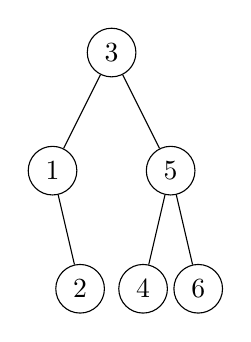
\begin{tikzpicture}[every node/.style={circle,draw},level 1/.style={sibling distance=15mm},level 2/.style={sibling distance=7mm}]\node{3} child { node{1} 
              child[missing]{}child{node{2}}}child { node {5} child { node {4} }child { node {6} }};\end{tikzpicture}                                
                \caption{}
                \label{fig:baum8}
            \endminipage
        \end{figure}
        
        Zuerst fügen wir in den leeren Baum unseren ersten Knoten $1$ ein (siehe Abbildung \ref{fig:baum1}).
        
        Als zweiten Schritt fügen wir die $3$ ein. Da $3 > 1$ ist, fügen wir diese als rechtes Kind ein (siehe Abb. \ref{fig:baum2}).
        
        Schritt Nummer drei ist das Einfügen von der $5$. Da sowohl $5>1$ und $5>3$ ist, wird die $5$ das rechte Kind der $3$ (Abb. \ref{fig:baum3}).
        
        Nun wird die Bedingung des AVL Baumes verletzt, da $3$ die Höhe $1$ hat, das theoretische linke Kind von $1$ jedoch die Höhe $-1$ hat. Wir rotieren links um die $3$ um die Eigenschaft wiederherzustellen (siehe Abb. \ref{fig:baum4}).
        
        Als fünften Schritt fügen wir eine $6$ in den Baum ein. $6>3$ und $6>5 \implies 6$ wird das rechte Kind von $5$ (siehe Abb. \ref{fig:baum5}).
        
        Als sechsten Schritt versuchen wir erneut eine $6$ in den Baum einzufügen, da unsere \textbf{\textsc{AVL-Insert}}-Prozedur keine Duplikate zulässt, bleibt der Baum unverändert (siehe Abb. \ref{fig:baum6}).
        
        Schritt $7$ ist es eine $4$ in den AVL Baum einzufügen. Es gilt $4>3$, aber $4<5$, weswegen die $4$ als linkes Kind der $5$ platziert wird (siehe Abb. \ref{fig:baum7}).
        
        Als letzten Schritt fügen wir eine $2$ hinzu. $2<3$, aber $2>1$, deshalb wird die $2$ zum rechten Kind der $1$. Somit wurden alle Schlüssel hinzugefügt und der AVL Baum ist komplett (siehe Abb. \ref{fig:baum8})). \hfill \qedsymbol

        \item  Zeigen Sie, für einen beliebigen AVL-Baum gilt: $n \leq 2^{h+1} - 1$ (2 Punkte)
        \begin{proof}
            Für vollständige Binärbäume der Höhe $h$ wissen wir dass diese $n = 2^{h+1} - 1$ Knoten haben. Jeder andere AVL-Baum der Höhe $h$ muss folglich weniger Elemente besitzen, sodass $n \leq 2^{h+1} - 1$ gilt.
        \end{proof}
        
        \item Zeigen Sie, für einen beliebigen AVL-Baum gilt: $(\frac{3}{2})^h \leq n$ (2 Punkte)
        \begin{behauptung}
            Für einen AVL-Baum der Höhe $h$ gilt $\frac{3}{2}^h < \phi^h \leq n$
        \end{behauptung}
        \begin{proof}
            Sei $N(h)$ die minimale Knotenanzahl eines AVL-Baumes der Höhe $h$. Wir stellen eine Rekurrenzgleichung mit $N(0) = 1$ und $N(1) = 2$ auf:
            Für $n\geq2$ sei $h_L$ und $h_R$ bezeichnen entsprechend die Höhe des linken- und rechten Teilbaums. Weil der Baum die Höhe $h$ hat, muss einer der Teilbäume die Höhe $h-1$ haben, angenommen es sei $h_L$.
            Um die Anzahl der Knoten zu minimieren, machen wir den anderen Teilbaum, $h_R$, so klein wie möglich. Wegen der AVL Eigenschaft folgt daraus $h_R = h-2$. Zählt man nun den Wurzelknoten, die Anzahl der Knoten im rechten- und linken Teilbaum bekommt man folgende Rekurrenzgleichung für die totale Anzahl an Knoten:
            \begin{align*}
                N(0) &= 1 \\
                N(1) &= 2 \\
                N(h) &= 1 + N(h_L) + N(h_R) \\
                &= 1 + N(h - 1) + N(h - 2).
            \end{align*}
            Wir stellen fest, dass die Anzahl der Blätter der Fibonacci-Reihe folgt. Da wir eine untere Schranke suchen, ignorieren wir den Term $+1$ der Wurzel.
            Also gilt $N(h) \geq \phi^h \approx 1.618^h$
            
            Folglich muss $N(h) < n$ sein, sodass gilt:
            \[
            \left(\frac{3}{2}\right)^h < \phi^h \leq n
            .\]
        \end{proof}
    \end{enumerate}
\end{question}

\begin{question}
    Beweisen oder widerlegen Sie folgende Aussagen zu ungerichteten Graphen:
    \begin{enumerate}
        \item Es gilt für $G = (V, E)$:
\[
\sum_{v \in V} deg(v) = 2|E|
\]
            (2 Punkte)
            \begin{proof}
                Sei $G$ ein kantenloser Graph mit mindestens $2$ Kanten. Für $G$ gilt $deg(V_i) = 2 \cdot 0 = 0$.
                
                Für jede Kante $e = (v_1, v_2)$, die wir hinzufügen, erhöhen wir den Grad für $v_1$ und $v_2$ um jeweils $1$.
                Da eine neue Kante immer $2$ Knoten verbindet, muss die Summe aller Grade immer doppelt so groß sein, wie die Anzahl der Kanten. Die Behauptung stimmt.
            \end{proof}
           
            
        \item Seien $v, w$ die einzigen beiden Knoten in $G = (V, E)$ mit ungeradem Grad, so sind $v$ und $w$ über einen Pfad in G verbunden.(2 Punkte) \\
            \emph{Hinweis: Nutzen Sie die Aussage aus Aufgabe a).}


            \emph{Beweis durch Widerspruch:}
            Seien $v$ und $w$ Knoten in zwei jeweils nicht zusammenhängenden Teilgraphen. Aus Aufgabe $4a$ wissen wir, dass $v$ nicht der einzige Knoten mit ungeradem Grad in seinem Teilgraph sein kann, daher muss es einen zweiten Knoten mit ungeradem Grad in diesem Teilgraph geben. Da $v$ und $w$ die einzigen Knoten mit ungeradem Grad sind, müssen beide in einem zusammenhängenden Teilgraph liegen. Folglich gibt es einen Pfad zwischen $v$ und $w$. \hfill\qedsymbol

\newpage
        \item $G = (V, E)$ ist zusammenhängend, wenn für alle Knoten $v \in V$ gilt:
\[
deg(v) \geq \left\lceil\frac{|V|-1}{2}\right\rceil
\]
            (2 Punkte)
            
            In der Vorlesung haben wir ungerichtete Graphen als schleifenfrei eingeführt (Foliensatz 5, Seite 3).
            
            Angenommen $G$ ist nicht zusammenhängend, dann existiert o.B.d.A. eine kleinste Zusammenhangskomponente $G_Z$:
            \begin{align*}
                G_Z &=(V_Z, E_Z) \\
                V_Z &\subsetneq V \\
                E_Z &= \{\{e_i, e_j\}\; |\; e_i, e_j \in V_Z\} \cap E \\
                |V_Z| &\leq \floor*{\frac{|V|}{2}}
            .\end{align*}
            Sei $deg(v)$ für alle $v \in V_Z$ maximal, dann wäre die Zusammenhangskomponente $G_Z$ ein vollständiger Graph $K_{|V_Z|}$ dann ist $\forall v \in V_Z$:
            \begin{align*}
                deg(v) &= |V_Z-1| \\
                 &= \abs*{\floor*{\frac{|V|}{2}}} = \floor*{\frac{|V|}{2}}\\
                 &< \floor*{\frac{|V|}{2}} + 1  = \ceil*{\frac{|V|}{2}}
            .\end{align*}
            Um die Formel aus der Behauptung erfüllen zu können, brauchen alle Knoten in der Zusammenhangskomponente $G_Z$ jeweils eine Kante mehr, da aber alle Knoten in $G_Z$ zu allen anderen Knoten in $G_Z$ eine Kante haben, müssen die neuen Kanten zu anderen Zusammenhangskomponenten gehen. Da das für alle Zusammenhangskomponenten gilt, muss $G$ zusammenhängend sein. \hfill \qedsymbol

\newpage
            Angenommen, man lässt Schleifen zu. Wir betrachten folgenden Graphen $G'$:
            
        \begin{figure}[ht]
            \minipage{0.2\textwidth}
            \centering
            \begin{align*}
                G' &=(V', E') \\
                V' &= \{a,b\} \\
                E' &= \{ \{a,a\}, \{b,b\} \}
            \end{align*}
            \endminipage
            \minipage{0.2\textwidth}
            \centering
            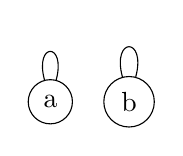
\begin{tikzpicture}[every loop/.style={}]
                \node[circle,draw] (a) at (0,0) {a};
                \node[circle,draw] (b) at (1,0) {b};
                
                \path (a) edge [loop above] node {} (a);
                \path (b) edge [loop above] node {} (b);
            \end{tikzpicture}
            \endminipage
        \end{figure}
            Da Schleifen den Grad eines Knotens um $2$ erhöht, gilt offensichtlich sowohl für $a$ als auch für $b$, dass
\[
    deg(a)=deg(b)=2 > \ceil*{\frac{|V'|-1}{2}} = \ceil*{\frac{1}{2}} = 1
\]
            , jedoch ist  $G'$ nicht zusammenhängend. $\lightning$
    \end{enumerate}
\end{question}

\begin{question}
\tikzset {
    treenode/.style={align=center,inner sep=0pt},
    % Black nodes
    node_black/.style={treenode,circle,white,font=\bfseries,draw=black,fill=black,text width=0.8cm},
    % Red nodes
    node_red/.style={treenode,circle,red,draw=red,very thick,text width=0.8cm},
    % Nil nodes
    node_nil/.style={treenode,rectangle,white,fill=black,minimum width=0.3cm, minimum height=0.3cm}
}
    \textbf{Bonusaufgabe}\\
    Im Kapitel 13-1 im Cormen wird der Rot-Schwarz-Baum, ein spezieller Binärbaum, definiert. Lies das Kapitel durch, und beantworte folgende Fragen zu dem Rot-Schwarz-Baum.
    \begin{enumerate}
        \item Geben Sie einen validen Rot-Schwarz-Baum an der aus folgenden Elementen besteht: $\langle1,5,9,10,13,16,20\rangle$ (1 Punkt)
        \begin{figure}[ht]
            \centering
            \begin{tikzpicture}[->,level distance=10mm,level 1/.style={sibling distance=20mm},level 2/.style={sibling distance=10mm},level 3/.style={sibling distance=6mm}]
                \node[node_black]{10}
                    child { node[node_red]{5}
                        child { node[node_black]{1}
                            child { node[node_nil]{} }
                            child { node[node_nil]{} }
                        }
                        child { node[node_black]{9}
                            child { node[node_nil]{} }
                            child { node[node_nil]{} }
                        }
                    }
                    child { node[node_red]{16}
                        child { node[node_black]{13}
                            child { node[node_nil]{} }
                            child { node[node_nil]{} }
                        }
                        child { node[node_black]{20}
                            child { node[node_nil]{} }
                            child { node[node_nil]{} }
                        }
                    }
                ;
            \end{tikzpicture}
            \caption{Lösung für Aufgabe 5a)}
        \end{figure}
        
        \newpage
        \item Zeigen Sie, dass in einem Rot-Schwarz Baum der längste einfache Pfad von einem beliebigen Knoten $x$ zu einem untergeordneten Blatt höchstens doppelt so lang sein kann wie zu einem anderen untergeordneten Blatt. (2 Punkte)
        
        \begin{figure}[ht]
            \tikzstyle{every node}=[circle,draw=black]
            \hfill
            \minipage[b]{0.2\textwidth}
            \centering
            \begin{tikzpicture}[->,level distance=10mm,level 1/.style={sibling distance=20mm},level 2/.style={sibling distance=10mm},level 3/.style={sibling distance=6mm}]
                \node[node_black]{$x$}
                    child { node[node_red]{}
                        child { node[node_black]{}
                            child { node[node_red]{}
                                child { node[node_nil]{y} }
                                child { node[node_nil]{} }
                            }
                            child { node[node_nil]{} }
                        }
                        child { node[node_black]{}
                            child { node[node_nil]{} }
                            child { node[node_nil]{} }
                        }
                    }
                    child { node[node_black]{}
                            child { node[node_nil]{} }
                            child { node[node_nil]{z} }
                    }
                ;
            \end{tikzpicture}
            \caption{(Teil-)baum\\ von schwarzem $x$}
            \endminipage\hfill
            \minipage[b]{0.29\textwidth}
            \begin{tikzpicture}[->,
            level 1/.style={sibling distance=36mm},
            level 2/.style={sibling distance=18mm},
            level 3/.style={sibling distance=10mm},
            level 4/.style={sibling distance=6mm}]
                \node[node_red]{$x$}
                child { node[node_black]{}
                    child { node[node_red]{}
                        child { node[node_black]{}
                            child { node[node_red]{}
                                child { node[node_nil]{y} }
                                child { node[node_nil]{} }
                            }
                            child { node[node_nil]{} }
                        }
                        child { node[node_black]{}
                            child { node[node_nil]{} }
                            child { node[node_nil]{} }
                        }
                    }
                    child { node[node_black]{}
                            child { node[node_nil]{} }
                            child { node[node_nil]{} }
                    }
                }
                child { node[node_black]{}
                    child { node[node_black]{}
                            child { node[node_nil]{} }
                            child { node[node_nil]{} }
                    }
                    child { node[node_black]{}
                            child { node[node_nil]{} }
                            child { node[node_nil]{z} }
                    }
                }
                ;
            \end{tikzpicture}
            \caption{Teilbaum von rotem $x$}
            \endminipage
        \end{figure}
        
        Wir erinnern uns an die Eigenschaften eines Rot-Schwarz Baums (RBT)
        \begin{enumerate}[label=\arabic*.]
            \item Jeder Knoten ist entweder \emph{rot} oder \emph{schwarz}.
            \item Die Wurzel ist \emph{schwarz}.
            \item Die Blätter (NIL-Knoten) sind \emph{schwarz}.
            \item Wenn ein Knoten \emph{rot} ist, dann sind seine beiden Kinder \emph{schwarz}.
            \item Jeder Knoten $x$ hat die selbe Schwarz-Höhe, d.h. das auf jedem Pfad von $x$ zu dessen Blätter gleich viele \emph{schwarze} Knoten sind.
        \end{enumerate}
        
        \emph{Behauptung:} Seien $p_s$ und $p_r$ Pfade von $x$ zu dessen Blätter. Dabei ist $p_s$ ein möglichst kurzer und $p_r$ ein möglichst langer Pfad. Ferner sei $h_s$ die Höhe des Pfades von $p_s$, dann gilt für $p_r$, dass dessen Höhe $h_r$ durch die Ungleichung $h_r \leq 2 \cdot h_s$ beschränkt ist. 
        \begin{proof}
        Da alle Pfade von $x$ zu dessen Blätter die selbe Schwarz-Höhe haben müssen (Eigenschaft 5), ist die Anzahl der schwarzen Knoten auf den Pfaden $p_r$ und $p_s$ gleich. Hierbei sieht man leicht, dass $p_s$ lediglich aus schwarzen Knoten besteht (Eigenschaft 1-3). Damit $p_r$ größtmöglich ist, kann nur an jeder zweiten Stelle des Pfades ein roter Knoten sein (Eigenschaft 4).
        
        Falls $x$ selbst schwarz ist, dann kann man nur höchsten $h_s$ rote Knoten in $p_r$ haben, womit $p_r$ dann $h_s + h_s = 2 \cdot h_s$ Knoten hat. Wenn $x$ rot ist, kann der nächste Knoten auf $p_r$ nicht auch rot sein (Eigenschaft 4). Wenn jeder andere zweite Knoten in $p_r$ rot ist, ergibt das $p_r$ dann $h_s + h_s - 1 \leq 2 \cdot h_s$. Falls ein Pfad von $x$ zu einem seiner Blätter weniger rote Knoten als $p_r$ hat gilt die Ungleichung erst recht.
        \end{proof}

        \item Was ist die größte Anzahl an internen Knoten, aus die ein Rot-Schwarz-Baum bestehen kann wenn die Schwarz-Höhe des Baumes $k$ ist? Was ist die geringste Anzahl? (2 Punkte)
        
        Bei einem RBT der Schwarz-Höhe $k$ ist die größte Anzahl der internen Knoten $2^{2k}-1$, wobei der Baum dann vollständig mit der Höhe $2k$ ist (insg. $2^{2k+1}-1$ Knoten) und $2^k$ NIL-Knoten hat. Jede zweite Ebene ist dabei rot.
        
        \[
        \underbrace{2^{2k+1}-1}_{\# gesamt}\quad -\underbrace{2^{2k}}_{\# NIL-Knoten} = \underbrace{2^{2k}-1}_{\# innere-Knoten} \hfill \textbf{(max)}
        \]
        
        Sei der RBT mit der Schwarz-Höhe $k$ vollständig und alle internen Knoten \emph{schwarz}. Dann ist dessen Höhe auch $k$ und für vollständige Binärbäume der Höhe $k$ gilt:
        
        \[
        \underbrace{2^{k+1}-1}_{\# gesamt}\quad -\underbrace{2^k}_{\# NIL-Knoten} = \underbrace{2^k -1}_{\# innere-Knoten} \hfill \textbf{(min)}
        \]
    \end{enumerate}
\end{question}


\end{document}
